\documentclass{modernsimplecv}
% try out different fonts: classic, fira, raleway, chivo
\usepackage[utf8]{inputenc}
\usepackage[margin=1cm, a4paper]{geometry}

% ------------------------------------------------------------------------------------
% you can try out different fonts here by commenting the following lines in and out
% -----------------------------------------------------------------------------------
\usepackage[default]{raleway}
%\usepackage[sfdefault]{FiraSans} %% option 'sfdefault' activates Fira Sans as the default text font\renewcommand*\oldstylenums[1]{{\firaoldstyle #1}}\normalfont
%\usepackage[familydefault,light]{Chivo} 
%\usepackage[sfdefault,light,condensed]{roboto}
%\usepackage[default]{cantarell}
%\usepackage[sfdefault]{AlegreyaSans}


\usepackage{beuron}
\usepackage{LobsterTwo}%if not suposed to be main font, load other main font after this



%------------------------------------------------------------------ Variablen

\newlength{\rightcolwidth}
\newlength{\leftcolwidth}
\setlength{\leftcolwidth}{0.48\textwidth}
\setlength{\rightcolwidth}{0.47\textwidth}

%------------------------------------------------------------------
\title{21I506_Resumae}
\author{\LaTeX{} Tony Alosius}
\date{December 2022}

\pagestyle{empty}
\begin{document}


\thispagestyle{empty}
%-------------------------------------------------------------



\tikz[remember picture,overlay] {%
\node[rectangle, fill=white, anchor=north, minimum width=\paperwidth, minimum height=5cm](header) at (current page.north){};%
}

\begin{minipage}[t]{0.21\textwidth}
\vspace{0pt} % Trick for alignment
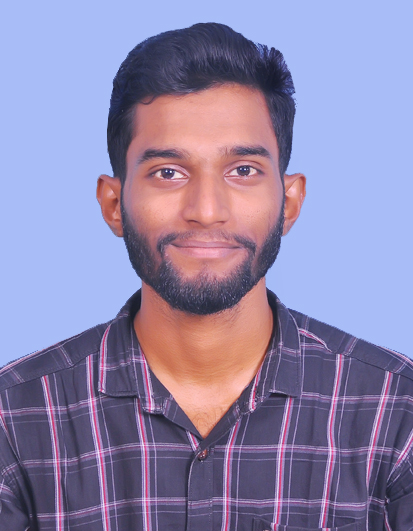
\includegraphics[width=\textwidth]{image.jpg}\hspace{1em}
\end{minipage}
\hfill
\begin{minipage}[t]{0.77\textwidth}
\vspace{0pt} % Trick for alignment
\begin{shaded*}

\begin{minipage}[t]{0.4\textwidth}
\vspace{0pt} % Trick for alignment
% here the fancy font can be taken out by removing \LobsterTwo
{\par\centering\huge\sans\bfseries{Tony Alosius}} \\[0.3cm]
\faGlobe~ Nationality: Indian\\
% \faBirthdayCake~ 10/10/1998 \\
\faMapMarker~ Krishnagiri, Tamil Nadu \\

{\small
\faGraduationCap~ {} Artificial Intelligence \\
\faCommentsO~ {Languages:} \emph{Tamil}, \emph{English}.}
\end{minipage}\hfill
\begin{minipage}[t]{0.55\textwidth}
\vspace{0pt} % Trick for alignment
\faPhone~ +91 8220552122 \\
\faAt~ \protect{tony.aloysius.77@gmail.com} \\

\faEnvelopeO~ TA Villa \\ 
\faMapMarker~ 3/329, Maniam Street, Kandhikuppam,\\
                Bargur, Krishnagiri,\\ 
                Tamil Nadu - 635108\\

%\aiAcademiaSquare 
\faFont~ \protect{https://kceai.com/tonyalosius} \\
\faGithub~ \protect{https://github.com/tonyalosius} \\
%\aiOrcid 
% \faCircle~ \protect{https://medium.com/@tony.aloysius.77} \\
\end{minipage}
\hfill
\end{shaded*}
\end{minipage}\\[15pt]


%------------------------------------------------

% hier muss die "unsichtbare" Überschrift rein, weil er sonst nicht die Paracols startet... komisch...
\subsection*{}
\vspace{-3em}

\setlength{\columnsep}{1.5cm}
\columnratio{0.48}[0.47]
\begin{paracol}{2}
\hbadness5000
%\backgroundcolor{c[1]}[rgb]{1,1,0.8} % cream yellow for column-1 %\backgroundcolor{g}[rgb]{0.8,1,1} % \backgroundcolor{l}[rgb]{0,0,0.7} % dark blue for left margin

\paracolbackgroundoptions

% 0.9,0.9,0.9 -- 0.8,0.8,0.8


\footnotesize
{

\small
\section*{Education}
\medskip
\begin{minipage}[t]{\leftcolwidth}
\begin{tabular}{r| p{0.6\textwidth} c}
    \cvevent{2021-2024}{B. Tech Artificial Intelligence \& Data Science}{Coimbatore}{Tamil Nadu}{Karpagam College of Engineering - CGPA:9.57}{} \\
    \cvevent{2017-2020}{B. Sc. Mathematics}{Dharmapuri}{Tamil Nadu}{Don Bosco College of Arts \& Science - CGPA-9.0}{} \\
    \cvevent{2015--2016}{Higher Secondary Certificate}{Krishnagiri}{Tamil Nadu}{Sri Vija Vidyalaya School - Percent: 96}{}\\
    \cvevent{2013--2014}{SSLC}{Krishnagiri}{Tamil Nadu}{Don Bosco School - Percent: 94.5}{}
    
\end{tabular}

\vspace{0.5em}

\small
\section*{Internships}
\medskip
\begin{tabular}{r| p{0.6\textwidth} c}
    \cvevent{Dec, 2021}{We\&Data}{Microsoft PowerBI}{}{Hands on virtual Internship on Microsoft PowerBI Ddata Visualization Tool}{} \\
    \cvevent{Dec, 2022}{TCS-iON}{Deep Learning}{}{Deep Learning technoques for Natural Language Processing}{} \\
    
\end{tabular}
\section*{Awards}
\medskip
\begin{tabular}{r| p{0.6\textwidth} c}
    \cvevent{2020}{Best Out-Going Student 2020}{Don Bosco College}{Dharmapuri}{Prestigious award for Overall Excellence throughout the 3 years of graduation in academics, co-curricular, extra-curricular and sports activities.}{} \\
    \cvevent{2017--2020}{Academic Proficiency Award}{Don Bosco College}{Dharmapuri}{Outstanding Academic Excellence in all the semesters}{} 
\end{tabular}
\end{minipage}



\vspace{3em}

\begin{minipage}[t]{\leftcolwidth}
\section*{Certifications}
\medskip
\begin{tabular}{r| p{0.6\textwidth} c}
    \cvevent{Coursera}{Google Data Analytics}{Professional Certificate}{KCE}{Skills  gain gained : Data cleaning, problem solving, critical thinking, data ethics, and data visualization through Presentations, Spreadsheets, SQL, Tableau and R Programming}{} \\
    \cvevent{}{Data Science Ethics}{Coursera}{KCE}{Getting to Know basic concerns while handling and manipulating the data}{} \\
    \cvevent{}{Amazon Web Services}{Coursera}{KCE}{Getting Started with Data Analytics on AWS an online course authorized by Amazon Web Services}{} \\
    \cvevent{}{Deep Learning using Tensorflow}{Professional Certificate}{KCE}{Introduction to TensorFlow for Artificial Intelligence, Machine Learning, and Deep Learning.}{}\\
    \cvevent{FreeCodeCamp}{Scientific Computing with Python}{Certification}{KCE}{Python fundamentals like variables, loops, conditionals, and functions.}{} \\
    \cvevent{}{Responsive Web Design}{Developer Certification}{KCE}{Skills  gain gained in this Responsive Web Design Certification,  HTML (Hypertext Markup Language) for content, and CSS (Cascading Style Sheets) for design.}{} \\
     \cvevent{Tableau}{Tableau Fundamentals}{Certification}{KCE}{Fundamentals of Tableau}{} \\
     \cvevent{Forage}{Tata Data Visualization}{Certification}{KCE}{Data Visualisation: Empowering Business with Effective Insights}{}
\end{tabular}
\end{minipage}
\vspace{2em}
\section{Declaration}

}
%-----------------------------------------------------------
\switchcolumn

\section{Objective} 
\medskip
\normalsize{
Focused and diligent pursuing graduate in artificial intelligence and data sciences looking to leverage in-depth knowledge in technical skills to drive success in the field of automation and business intelligence team and Looking for a challenging role in a reputable organization to utilize all my skills gained for the growth of the organization as well as to enhance my knowledge about new and emerging trends in the IT sect.
}

\medskip
\section{Programming Languages} 
{\small
}
\medskip

\begin{skillsection}{\rightcolwidth}
    \medskip
    \cvitem{\faStar\faStar\faStar\faStar\faStar}{Python}
    \medskip
    \cvitem{\faStar\faStar\faStar\faStarO\faStarO}{C Programming}
    \medskip
    \cvitem{\faStar\faStar\faStar\faStar\faStarO}{R}
    \medskip
    \cvitem{\faStar\faStar\faStar\faStarO\faStarO}{Java}
    \medskip
    \cvitem{\faStar\faStar\faStar\faStar\faStar}{HTML}
    \medskip
    \cvitem{\faStar\faStar\faStar\faStar\faStar}{CSS}
\end{skillsection}

\section*{Technical Skills}
\medskip
\begin{tabular}{>{\footnotesize\bfseries}r >{\footnotesize}p{0.7\textwidth}}
    \medskip
    \faFutbolO & \emph{Database Management} \\
    \medskip
    \faFutbolO & \emph{Data Structures}\\
    \medskip
    \faFutbolO & \emph{Machine Learning} \\
    \medskip
    \faFutbolO & \emph{Deep Learning}\\
    \medskip
    \faFutbolO & \emph{Computer Vision}\\
    \medskip
    \faFutbolO & \emph{Drone Programming}
\end{tabular}

\section*{Tools}
\medskip
\begin{tabular}{>{\footnotesize\bfseries}r> {\footnotesize}l >{\footnotesize\bfseries}r >{\footnotesize}l p{0.7\textwidth}}
    \smallskip
    \faFutbolO & \emph{R Studio} & \faFutbolO & \emph{Visual Studio} \\
    \smallskip
    \faFutbolO & \emph{Microsoft PowerBI} & \faFutbolO & \emph{Google Colab}\\
    \smallskip
    \faFutbolO & \emph{Tableau} & \faFutbolO & \emph{Git \& Github}\\
    \smallskip
    \faFutbolO & \emph{Microsoft Spreadsheet} & \faFutbolO & \emph{Android Studio}\\
    \smallskip
    \faFutbolO & \emph{Pycharm} & \faFutbolO & \emph{XAMPP}\\
    \faFutbolO & \emph{Looker Studio} \\
    \smallskip
\end{tabular}


\begin{minipage}[t]{\rightcolwidth}
\section*{Projects}
\medskip
\begin{tabular}{r| p{0.6\textwidth} c}
    \cvevent{December 2021}{Fish Species Detection}{Smart India Hackathon}{India}{Animal Species Detection - Fish Species Detection App for Fisher men in order to segregate fish by species.}{} \\
    \cvevent{May 2022}{Talking Dictionary}{Academic Project}{KCE}{Vocabulary program which spells out the meaning of the word.}{} \\
    \cvevent{August 2022}{Virtual Mouse}{Computer Vision}{KCE}{\bold OpenCv -- Virtual Mouse Cursor Controller through which we can Control the moves of the cursor through our finger Landmarks and eyes }{}\\
    \cvevent{October 2022}{Data Visualization}{Tableau}{KCE}{\bold Analysis of various data and drawing insights from it through Visualization.}{}\\
    \cvevent{August 2022}{Nvidia DGX}{MIG}{KCE}{\bold Installing and Configuting Nvidia DGX A100 Workstaion for Deep Learning Programming }{}\\
    \cvevent{November 2022}{Drone Programming}{DjiTellopython}{KCE}{Dji Tello Drone programming project for Survillence using Deep Learning Techniques.}{}\\
    \cvevent{December 2022}{Agricultural Drone}{Computer Vision}{KCE}{OpenCv -- Programming a drone to perform the Leaf Disease Detection }{}
\end{tabular}
\end{minipage}
\end{paracol}


\begin{minipage}[t]{\textwidth}
\normalsize{ I here by declare that all the information in this resume is right and truthful to the best of my knowledge and faith.}
\end{minipage}
\vfill{} % Whitespace before final footer

%----------------------------------------------------------------------------------------
%	FINAL FOOTER
%----------------------------------------------------------------------------------------
\setlength{\parindent}{0pt}
\begin{minipage}[t]{\textwidth}
\begin{center}\fontfamily{\sfdefault}\selectfont \color{black!70}
{\small Tony Alosius \icon{\faAt}{black}{} \protect{tony.aloysius.77@gmail.com} \icon{\faMapMarker}{black}{} Krishnagiri \icon{\faPhone}{black}{} +91 8220552122 

}
\end{center}
\end{minipage}

\end{document}
